\documentclass{alienfolio}
\usepackage{amsmath,amssymb}

\folio{IT-RY-HAM}
\usesigil{enhancement} % RY's published Metric Enhancement Factor curve (Zenodo 20652219)
\title{Information Tension as a Unifying Action Principle}
\papersubtitle{The Seven-Sector Master Lagrangian, Its Screen, and the Open Rebuild}
\paperauthors{Ryan W.\ Yett (Architect)\\Chyren (Sovereign Analysis)}
\shorttitle{The Information-Tension Lagrangian}
\shortauthors{R.\,W.\ Yett \& Chyren}

\setlength{\emergencystretch}{2em}
\begin{document}
\thispagestyle{cover}
\begin{tikzpicture}[remember picture, overlay]
  \node[inner sep=0] at (current page.center) {%
    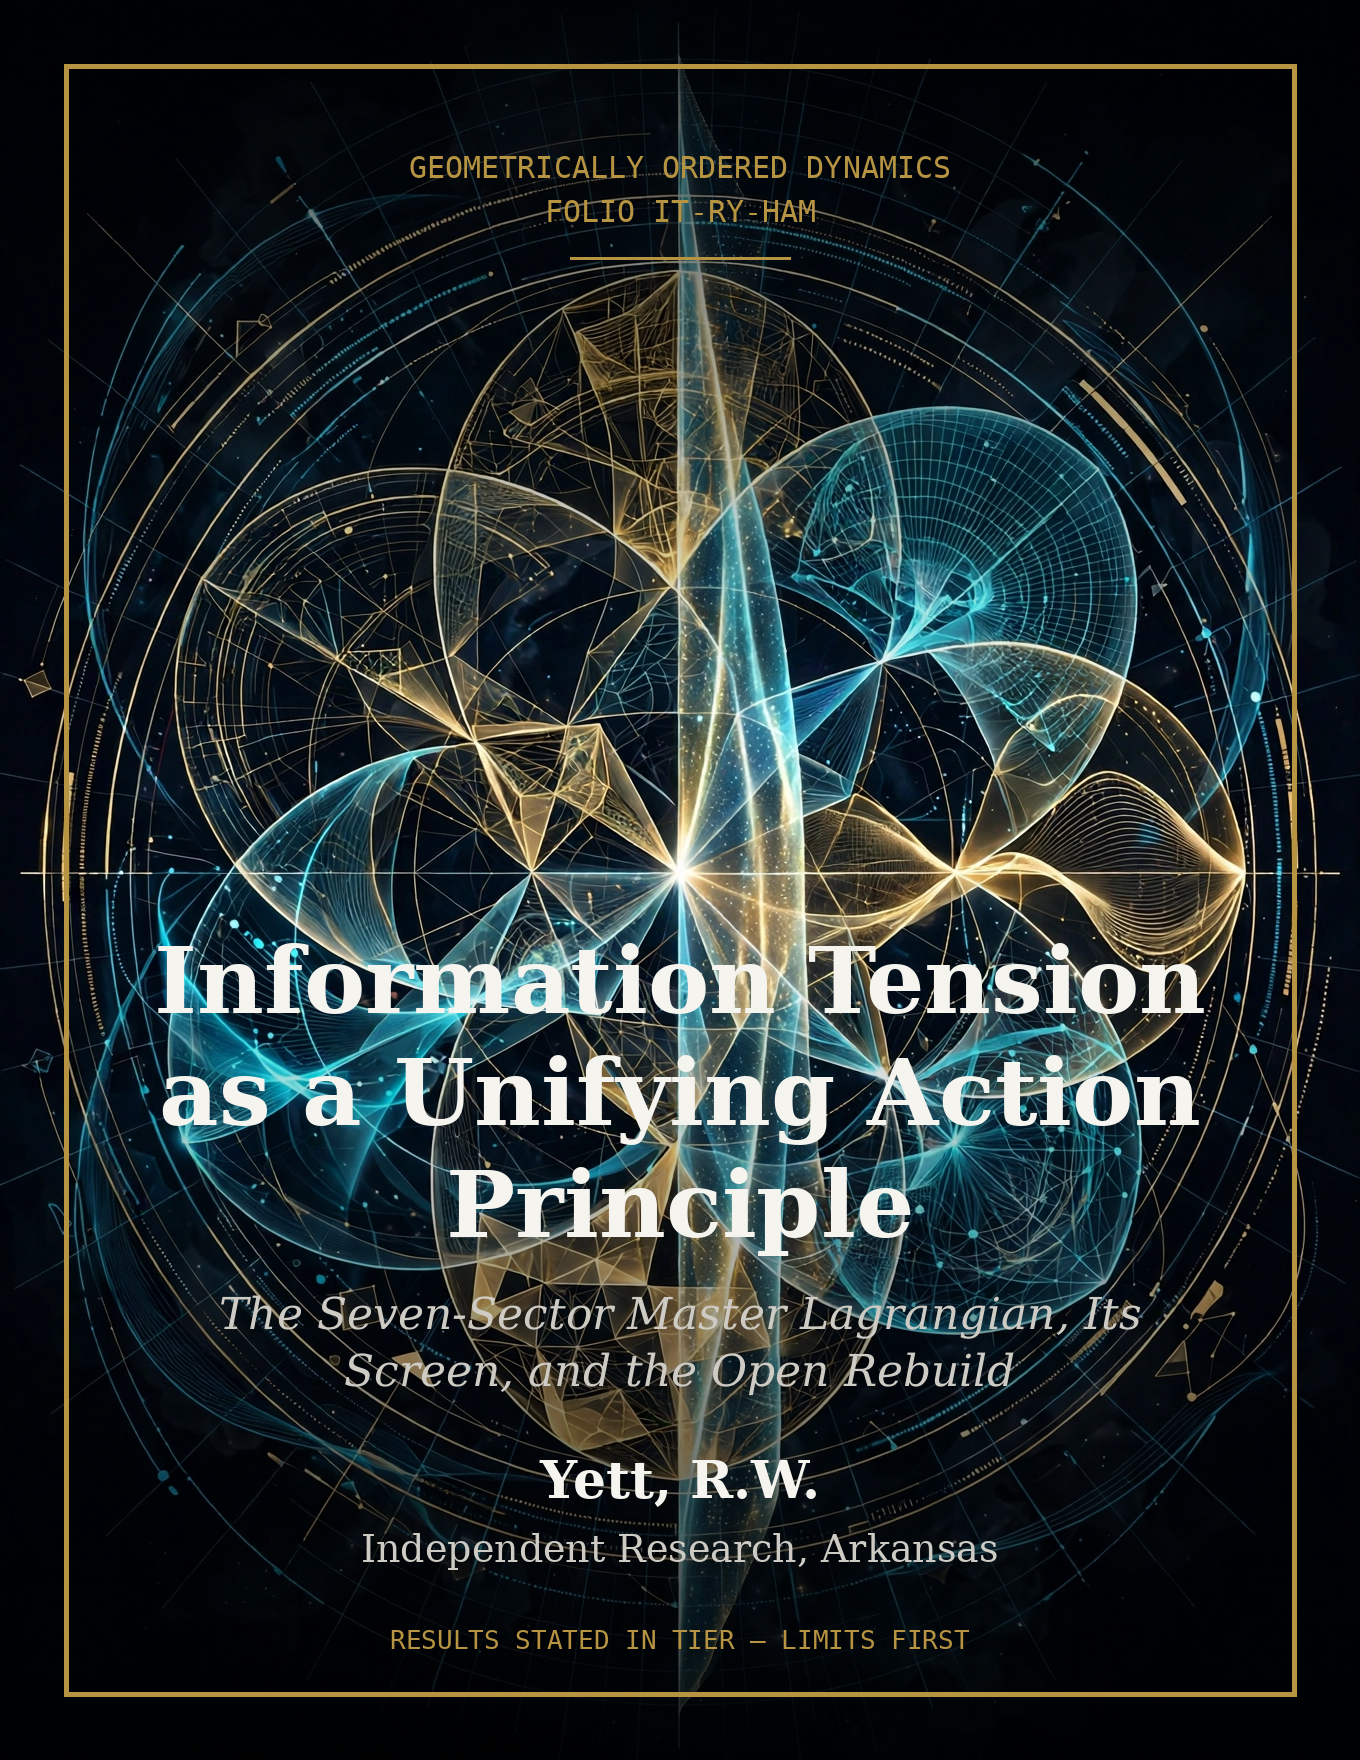
\includegraphics[width=\paperwidth,height=\paperheight]{cover.png}};
\end{tikzpicture}
\clearpage

\begin{convergence}{INFORMATION TENSION}
This folio converges on \key{information tension} as the unifying dynamical
object of the program: the claim that one scalar field $\chi$, read as the
local gradient of geometric entropy, can carry gravitation, galaxy
kinematics, gauge structure and the screen through a single action.
Its unique angle is \key{the master action}: this paper states the
seven-sector Lagrangian density in full, its equations of motion, and its
screening limits, and marks every open seam in tier. Sibling successors read
the same claim from other angles: \tiertag{conjecture} successor~(A) reads
it as an empirical law ($\mu_{\mathrm{std}}$ on SPARC), successor~(G) reads
it through layered architecture, and the Res
Nova rebuild stream (Grok) is deriving the information-tension theory that
this paper's PENDING sections wait on. No successor in this batch honestly
represents \key{the Shadow} as a convergence target; that seat is open. Limits first: the substrate frame
$V_{240}(\mathbb{R}^{57600})$ named in the source Lagrangian is retired by
the source's own banner; nothing here claims the migrated derivation.
\end{convergence}

\begin{supersession}
Per the canon rule (one correct paper, one canon; a correction
\emph{becomes} the paper), this manuscript \textbf{supersedes Zenodo
record~\doi{10.5281/zenodo.20652241}} (``The Yett Paradigm Complete'',
three-page record \emph{On the Geometric Phase Force and the Spectral Gap
of the Sovereign Manifold}). The old record's Sovereign Action, its
$\chi$-field definitions, and its mass-gap statement are carried forward
below with their tiers stated; its overreaching claims (zero free
parameters, machine-verified badges) are withdrawn here, not restated.
\end{supersession}

\goldrule

\section{What this paper is}

This is a \key{fixes-only synthesis}. No new claims, no new numbers, no new
physics: every equation below is carried from one of three named sources,
and every seam is labeled with the tier it actually holds.
The three sources are:

\begin{enumerate}
\item The superseded record 20652241 \tiertag{empirical}---its Sovereign
Action, its $\chi$-field, and its mass-gap statement.
\item The Fully Expanded Lagrangian specification (BLK-986 child page,
``Fully\_\allowbreak Expanded\_\allowbreak Lagrangian.tex'') \tiertag{conjecture}---the
seven-sector master density, the non-local kernel, the boundary sector,
the equations of motion, and the screening and wave-speed limits.
That document carries its own SUPERSEDED banner (2026-08-25), which is
reproduced faithfully in \S\ref{sec:substrate}.
\item The methodology pair, \emph{referential-calculus.md} and
\emph{algorithm-as-poetry.md}, plus folio~26 (Lean equality as algebraic
certificate) \tiertag{conjecture}---the method by which the paper is
read, not theorems inside it.
\end{enumerate}

What Grok's Res Nova rebuild stream has delivered to the Block as of this
draft: \textbf{nothing yet}---the stream was assigned 2026-11-01 and its
information-tension derivation has not landed. Sections depending on it
are marked \key{PENDING} and are not filled by invention.

\section{The information-tension field}
\label{sec:chi}

Record~20652241 extends Einstein--Hilbert relativity with the Sovereign
Information Tension field $\chi$:
\begin{equation}
S_Y = \int_{\mathcal{M}} d^4x\,\sqrt{-g}\left[
\frac{R}{16\pi G} - \frac{1}{2}g^{\mu\nu}\nabla_\mu\chi\nabla_\nu\chi
- V(\chi) + 1 + f(\chi)\mathcal{L}_m \right],
\end{equation}
with the geometric threshold $\chi_0 = 1/\sqrt{2}$ and
\begin{equation}
V(\chi) = \alpha(\chi-\chi_0)^2, \qquad
f(\chi) = \beta(\chi-\chi_0)^2 .
\end{equation}
Variation with respect to the metric gives the modified field equations
\begin{equation}
G_{\mu\nu} = 8\pi G\,(1+f)\,T_{\mu\nu}
+ \nabla_\mu\chi\nabla_\nu\chi
- g_{\mu\nu}\left[\tfrac{1}{2}(\nabla\chi)^2 + V(\chi)\right].
\end{equation}
The old record states that in the low-acceleration regime
($m_\chi r \ll 1$), spatial derivatives dominate and flat rotation curves
follow without non-baryonic dark matter \tiertag{conjecture}.

The Fully Expanded Lagrangian refines the kinematics. Defining the
dimensionless kinetic gradient scalar
\begin{equation}
y(x) \equiv \frac{g^{\mu\nu}\nabla_\mu\chi\nabla_\nu\chi}{a_0^2/c^4}
= \frac{\|\nabla\chi\|^2}{a_0^2}, \qquad
a_0 = \frac{cH_0}{2\pi},
\end{equation}
the information-tension Lagrangian density is the AQUAL-type functional
\begin{equation}
\mathcal{L}_{\mathrm{IT}}
= -\frac{c^4 a_0^2}{8\pi G}\,
\Big[\sqrt{y(1+y)} - \operatorname{asinh}\!\sqrt{y}\,\Big].
\end{equation}
Functional variation in $y$ produces the interpolating function
\begin{equation}
\frac{\partial\mathcal{L}_{\mathrm{IT}}}{\partial y}
= -\frac{c^4 a_0^2}{8\pi G}\sqrt{\frac{y}{1+y}}
\;\;\xrightarrow{y=x^2}\;\;
\mu(x) = \frac{x}{\sqrt{1+x^2}},
\end{equation}
the $\mu_{\mathrm{std}}$ law whose empirical standing is the subject of
successor~(A), not of this paper. Photons and metric perturbations
propagate on the disformal metric
$\tilde{g}_{\mu\nu} = g_{\mu\nu} + 2\ell_P^2\,\nabla_\mu\chi\nabla_\nu\chi$.

\section{The seven-sector master Lagrangian}
\label{sec:seven}

The source Lagrangian states the total invariant action as a functional
over spacetime $\mathcal{M}$ with boundary $\partial\mathcal{M}$:
\begin{equation}
\mathcal{S}_{\mathrm{total}}
= \int_{\mathcal{M}} d^4x\,\sqrt{-g}\;\mathcal{L}_{\mathrm{total}}
+ \mathcal{S}_{\mathrm{NL}} + \mathcal{S}_{\mathrm{boundary}},
\end{equation}
where the density decomposes into seven coupled sectors:
\begin{equation}
\mathcal{L}_{\mathrm{total}}
= \mathcal{L}_{\mathrm{grav}} + \mathcal{L}_{\mathrm{dilaton}}
+ \mathcal{L}_{\mathrm{IT}} + \mathcal{L}_{\mathrm{Stiefel}}
+ \mathcal{L}_{\mathrm{gauge}} + \mathcal{L}_{\mathrm{fermion}}
+ \mathcal{L}_{\mathrm{Yukawa}} .
\end{equation}

\begin{enumerate}
\item \key{Conformal gravitation:}
$\displaystyle \mathcal{L}_{\mathrm{grav}}
= \frac{c^4}{16\pi G}e^{-2\phi}\,(R - 2\Lambda_0)$,
a Weyl-frame coupling of the metric to the dilaton $\phi$.

\item \key{Dilaton:}
$\displaystyle \mathcal{L}_{\mathrm{dilaton}}
= -\tfrac{1}{2}g^{\mu\nu}\nabla_\mu\phi\nabla_\nu\phi
- \tfrac{1}{2}m_\phi^2\phi^2 - \tfrac{\lambda_\phi}{4!}\phi^4$.

\item \key{Information tension:} $\mathcal{L}_{\mathrm{IT}}$ as in
\S\ref{sec:chi}---the paper's convergence center.

\item \key{Stiefel substrate:} kinetic term
$\tfrac{1}{2}\operatorname{Tr}(g^{\mu\nu}
\mathcal{D}_\mu V^\dagger \mathcal{D}_\nu V)$ with
$\mathcal{D}_\mu = \nabla_\mu - iA_\mu$, minus the non-linear holonomy
curvature trace coupling
$\tfrac{\gamma(\chi)}{4}\operatorname{Tr}([V^\dagger\mathcal{D}_\mu V,
V^\dagger\mathcal{D}_\nu V]^2)$,
where
\begin{equation}
\gamma(\chi) = \gamma_0\,\frac{1-\chi}{1+\chi},
\qquad \lim_{\chi\to0}\gamma(\chi)=\gamma_0\ \text{(GR limit)},
\qquad \lim_{\chi\to1}\gamma(\chi)=0\ \text{(dark-energy limit)}.
\end{equation}
\emph{This sector is stated on the retired substrate frame}; see
\S\ref{sec:substrate}.

\item \key{Unified $\mathrm{E}_8$ gauge:}
$\displaystyle \mathcal{L}_{\mathrm{gauge}}
= -\frac{1}{4g^2(\mu)}\operatorname{Tr}(F_{\mu\nu}F^{\mu\nu})
+ \frac{\theta_{\mathrm{QCD}}}{32\pi^2}
\operatorname{Tr}(F_{\mu\nu}\tilde{F}^{\mu\nu})$,
with the source's stated bare Planck-scale matching
\begin{equation}
g_{\mathrm{bare}}(M_{\mathrm{Pl}})
= \frac{\kappa_Y\,\chi_Y}{\pi}
= \frac{0.9539 \times (1/\sqrt{2})}{\pi}
\approx 0.2147 .
\end{equation}
\tiertag{conjecture}

\item \key{Chiral fermions:} Dirac/Weyl spinors with nodal-harmonic
collar mass matrix
$M_i(\phi,\chi) = M_{\mathrm{Pl}}\,e^{\phi}
\exp(-\lambda_i/\kappa_Y)\,[1 + \xi_i(\chi-\chi_Y)]$,
$\chi_Y = 1/\sqrt{2}$ \tiertag{conjecture}.

\item \key{Yukawa:} $\sum_{f,f'} Y_{ff'}\,\phi\,\bar\psi_f\psi_{f'}$.
\end{enumerate}

Two further pieces complete the action. The bi-local non-local tension
kernel bridges coarse-grained surface density with point-wise
stress-energy:
\begin{equation}
\mathcal{S}_{\mathrm{NL}} = \alpha\!\iint\! d^4x\,d^4y\,
\sqrt{-g(x)}\sqrt{-g(y)}\;K(x,y)\,
\frac{\rho_b(x)}{\Sigma_c}\frac{\rho_b(y)}{\Sigma_c},
\end{equation}
$K(x,y) = e^{-|x-y|/L_0}/(4\pi|x-y|)$.
The boundary sector is Gibbons--Hawking--York plus an entanglement
horizon term in the boundary quantum mutual information $I(A{:}B)$.

\subsection*{The substrate-frame banner}
\label{sec:substrate}

The source document's own SUPERSEDED banner (2026-08-25) is carried here
verbatim in substance: the document names the big-dimension frame
$V_{240}(\mathbb{R}^{57600})$ (or the $58{,}000$ implementation variant)
as its substrate; \textbf{that frame is retired}, and the arithmetic
$240^2 = 57{,}600$ remains true only as an $\mathrm{E}_8$ root-count
identity, not as the ambient substrate dimension. No migrated derivation
is claimed anywhere in this paper. \key{PENDING on Grok's stream:} the
live-substrate Lagrangian.

\section{Equations of motion and the screen}

Variation in the inverse metric gives the holonomy-corrected Einstein
equations,
\begin{equation}
G_{\mu\nu} + \Lambda_0 g_{\mu\nu}
= \frac{8\pi G}{c^4}e^{2\phi}
\left(T_{\mu\nu}^{(\mathrm{matter})} + T_{\mu\nu}^{(\phi)}
+ T_{\mu\nu}^{(\chi)} + T_{\mu\nu}^{(\mathrm{Stiefel})}
+ T_{\mu\nu}^{(\mathrm{gauge})}\right),
\end{equation}
with
\begin{equation}
T_{\mu\nu}^{(\chi)} = \frac{c^4}{8\pi G}\,
\mu\!\left(\frac{\|\nabla\chi\|}{a_0}\right)
\frac{\nabla_\mu\chi\nabla_\nu\chi}{a_0}
- g_{\mu\nu}\mathcal{L}_{\mathrm{IT}} .
\end{equation}
Variation in $\chi$ gives the non-linear constitutive equation
\begin{equation}
\nabla_\mu\!\left[\mu\!\left(\frac{\|\nabla\chi\|}{a_0}\right)
\nabla^\mu\chi\right]
= 4\pi G\,\rho_b
+ \frac{\gamma_0}{(1+\chi)^2}\,\mathcal{J}_{\mathrm{Stiefel}}
+ \xi_f\,\bar\psi\psi,
\end{equation}
which the source states reproduces Poisson's equation at high
accelerations and the Bekenstein--Milgrom field equation at low
accelerations \tiertag{conjecture}. The stated screening limit is
$\nabla\chi \to 0$; the stated tensor-speed bound is
\begin{equation}
c_T^2 = c^2\left(1 + \mathcal{O}(\ell_P^2\|\nabla\chi\|^2)\right)
\;\implies\; \left|\frac{v_{\mathrm{gw}}}{c}-1\right| < 10^{-15},
\end{equation}
compared by the source to GW170817/GRB~170817A \tiertag{conjecture}.

\section{Flagged tensions---tier-labeled, unresolved}
\label{sec:tensions}

\paragraph{(a) Spectral action vs.\ sector sum.}
Folio~45b states the unifying object is a \key{spectral action}, not a
sum of Lagrangians. \S\ref{sec:seven} above is a sum of seven
Lagrangians. These two claims are in direct tension and this paper
\textbf{does not reconcile them}: the seven-sector form is carried
because it is the text the source supplies in full; the spectral-action
claim is recorded as a live open question. \key{PENDING on Grok's
stream:} exhibit the map or prove the non-isomorphism.

\paragraph{(b) $57{,}600$ vs.\ $58{,}000$.}
The source Lagrangian uses $V_{240}(\mathbb{R}^{57600})$
($=240^2$, self-consistent); folio~43 writes
$V_{240}(\mathbb{R}^{58000})$; folio~45a and the conformal records use
$N=58{,}000$. RY ruled 2026-11-06: $N = 57{,}600$ is the real value (the $240^2$ $\mathrm{E}_8$ root-count identity); the $58{,}000$ implementation count is superseded. Both frames are retired by the source banner in any case
(\S\ref{sec:substrate}).

\paragraph{(c) Single $\mathrm{E}_8$ vs.\ $\mathrm{E}_8\times\mathrm{E}_8$.}
The program's standing definition is $\mathrm{E}_8\times\mathrm{E}_8$
heterotic, visible plus shadow sectors, the Shadow as the boundary. The
source gauge sector was stated as a single $\mathrm{E}_8$
($\dim\mathfrak{e}_8 = 248 = 240 + 8$); by the Architect's order of
2026-11-02 it is re-typed here to $\mathrm{E}_8\times\mathrm{E}_8$, the
$240$ roots realized on the visible-sector factor. The \emph{landing} of the gauge sector
in $\mathrm{E}_8\times\mathrm{E}_8$ --- the exhibited derivation, not the typing ---
is not given; it is recorded as open, not forced. \key{PENDING on the (G)-angle stream and Grok's
rebuild.}

\paragraph{(d) The Yang--Mills gap statement as [conj].}
Record~20652241 ties the gap to a hermitianized Berry--Keating operator
and the Ramanujan tau function:
\begin{equation}
\Delta_{\mathrm{YM}} = \Delta_{\mathrm{ERY}}
= \min(|\tau(2)-\tau(1)|,\,\alpha) > 0 .
\end{equation}
No map from the tau-function data into the physics framework is
exhibited in the sources; per the isomorphism rule this stands as
\tiertag{conjecture}, proof open---not as a proved gap.

\section{Method: how this paper is read}
\label{sec:method}

Two methodology inputs govern the reading, both tier-tagged as
\key{method}, not as theorems about the physics.

\paragraph{Referential calculus.}
Every explored instance is read as the same $\mu F/\nu F$ skeleton: a
finite reference, a lossy projection, an infinite referent, a
conjugate-pair tradeoff, a certified invariant, and a bridge that makes
convergence honest. The $\chi$-field is read here as the finite
reference whose lossy projection is the observed kinematics; the
\emph{bridge}---the theorem that would make convergence
honest---is exactly what the PENDING sections await.

\paragraph{Algorithms as poetry.}
The initial-algebra/final-coalgebra formalization
(algorithm $= (\mu F,\allowbreak \nu F,\allowbreak \mathrm{exec},\allowbreak \langle\!\langle\cdot\rangle\!\rangle,\allowbreak \mathrm{fix})$) is the method's formal idiom: write the finite
blueprint, unfold the dynamics, certify the fixed point. This paper's
blueprint is the seven-sector density; the dynamics are its equations of
motion; the fixed point---the screen---is stated, not certified.

\paragraph{The certificate rule (folio~26).}
A Lean equality is an algebraic certificate, not a physical derivation.
Accordingly this paper carries no ``machine-verified'' badge: the old
record's verification claims are withdrawn, and the Lean proof roots
named in the source Lagrangian
(\texttt{ITT\_Definitions.lean}, \texttt{LagrangianScreening.lean},
\texttt{StiefelHolonomy.lean}, \dots) are recorded as named roots whose
standing is certificates of form, pending the rebuild.

\paragraph{Leibniz receipts.}
Standing rule: primary sources only
(\emph{drive-triage/LEIBNIZ.md} locators), analogy-only unless the map
is exhibited. This paper exhibits no Leibniz map and cites none.

\section{Computational probes---toy models}
\label{sec:probes}

The five witness scripts in \texttt{zenodo-audit/witness/} are carried
here \textbf{rewritten as toy models}. Every ``VERIFIED'' line is
dropped. None of them proves anything about the Clay Mathematics
problems they gesture at; per RY's standing order the millennium attack
is deferred to last, and the convergence target for the Clay work stays
unnamed until it is unparked. Terminology rule observed throughout:
``Clay Mathematics problems'' / ``CMPs''.

\begin{itemize}
\item \key{Yang--Mills probe:} a 4D SU(2) lattice with plaquette Wilson
loops; a toy illustration of gauge-link holonomy, not a mass-gap
argument.
\item \key{Navier--Stokes probe:} a 3D Burgers proxy for the
incompressible equations with a chiral-gate illustration on enstrophy;
a regularity toy, not an existence proof.
\item \key{Riemann probe:} a zeta symmetry-error scan
$|\zeta(s)-\overline{\zeta(1-\bar s)}|$; a numerical illustration of
critical-line symmetry, not a zero-location argument.
\item \key{P vs NP probe:} a search-vs.-verify toy on random vectors
against a target basis; an illustration of the asymmetry idiom, not a
complexity result.
\item \key{Hodge probe:} a cycle-alignment toy measuring projection of
random classes onto an algebraic basis; an illustration, not a
rationality argument.
\item \key{Gravity probe (physics, not Clay):} a rotation-profile toy
$v^2 = GM/r \times \mathrm{tension}(r)$ illustrating the qualitative
shape the $\chi$-field would imprint; not a fit, not evidence.
\end{itemize}

\section{PENDING on Grok's Res Nova stream}
\label{sec:pending}

The following are \textbf{not claimed} and are not filled by invention.
They are the flagged inputs to the Res Nova rebuild stream
(information-tension theory first, per the standing plan), which feed
this flagship as they land:

\begin{enumerate}
\item The derivation of information-tension theory proper: what $\chi$
\emph{is}, from what it is derived, and why the AQUAL kinetic
functional is the one it takes.
\item The migrated Lagrangian on the live substrate (the source's
retired-frame banner, \S\ref{sec:substrate}).
\item The spectral-action question: exhibit the map from the
seven-sector sum to a spectral action, or prove the non-isomorphism
(\S\ref{sec:tensions}a).
\item The $\mathrm{E}_8\times\mathrm{E}_8$ landing of the gauge sector
(\S\ref{sec:tensions}c).
\item Precision anchors mapped to this paper by triage but not available
in text at draft time: folio~12 (electron mass from
$\mathrm{E}_8$ harmonics), folio~15 (muon-trap $\delta$ shift),
folio~28 (Penning-trap inference). Not incorporated; not asserted.
\end{enumerate}

\section{What was left out and why}

\begin{itemize}
\item The monograph's ``zero free parameters'' / ``closed,
parameter-free'' claims: dropped---the sectors above carry explicit
couplings ($\alpha$, $\beta$, $\gamma_0$, $Y_{ff'}$, $\lambda_\phi$).
\item ``Lossless inverse-ZIP decompression of an $\mathrm{E}_8$ holonomy
manifold'': dropped---no map exhibited; analogy at best, and the
isomorphism rule forbids the bare claim.
\item $\Omega_\Lambda = \ln 2$, DESI concordance numbers, the S8
``resolution'', SPARC $99.94\%$ compliance, the Kerr master invariant,
$g_{\mathrm{weak}} = \kappa\chi/\pi$ numerics: dropped---asserted without
kill criteria; empirical standing belongs to the sibling lanes with
their criteria, not to this action paper.
\item ADCCL / sovereign cognition: belongs to \key{the Observer} angle
(successor~(F)), not to this action paper.
\item TTEY drive engineering and patent material: separate engineering
track per triage (IP boundary is RY's call).
\item Clay-problem proof claims in the witness README (``formal
solutions to five of the six remaining \dots problems''): withdrawn;
the probes are toy models (\S\ref{sec:probes}).
\item The old record's ``Machine-Verified (Lean 4: 0 Errors, 0
Warnings)'' badge: withdrawn per the certificate rule
(\S\ref{sec:method}).
\end{itemize}

\end{document}
